Brindar una buena experiencia de usuario en una aplicación puede llegar a ser un gran desafío donde existen varios elementos que afectan directamente, como el \textbf{diseño}, ya que es importante jugar un buen estilo, de carácter agradable, y con animaciones amigables. El \textbf{rendimiento}, donde la aplicación debe desempeñar una buena fluidez de respuesta y \textbf{correctitud}, que se contemple una interfaz que tenga sentido con la funcionalidad de la misma.

Cuando entramos en el área web, nuestro caso una aplicación web, llegan algunos desafíos adicionales como aplicar soporte de diseño para variedad de densidades de pantallas y versiones de navegadores web, esto se debe a que nuestra aplicación estará expuesta en la web, donde puede ser accedida desde tabletas, móviles, computadores de escritorio, televisores, y cualquier dispositivo que tenga conexión a internet y un navegador. También el peso de la aplicación, incluyendo códigos, fuentes e imágenes impacta considerablemente al tiempo de espera para conexiones lentas a internet.

En este capítulo presentaremos herramientas que nos facilitarán el trabajo para lidiar las problemáticas mencionadas segmentando la aplicación por: arquitectura, diseño y utilidades extras a emplear. Cabe acotar que para el manejo de estas herramientas es necesario tener conocimiento sobre JavaScript, TypeScript\footnote{TypeScript \url{https://www.typescriptlang.org/}} (subconjunto de JavaScript con un sistema de tipos más robusto), CSS y HTML.

\section{Arquitectura}

La aplicación adoptará una arquitectura llamada \textit{Single-page Aplication} \cite{WikiSPA} (SPA) que significa aplicación de una página, donde se busca englobar toda la aplicación en una vista, logrando cargar la base de la aplicación completa y luego dinámicamente mediante JavaScript hacer la transición de las vistas. La gran ventaja que podemos sacar de SPA es la fluidez de la aplicación entre cambios de vistas, ya que todos estos elementos ya fueron cargados previamente. Por contraparte, la carga inicial suele ser pesada por traerse elementos de más, pero de igual forma esta puede optimizarse para traer solo los recursos necesarios.

Mayormente nuestra aplicación tendrá comunicación casi constante con un API que nos ofrecerá cantidades de datos para nosotros transmitir visualmente, por lo tanto manejaremos peticiones HTTP\footnote{HTTP: es el protocolo de comunicación que permite las transferencias de información en la World Wide Web.} (Hypertext Transfer Protocol) con AJAX \cite{AJAX} (Asynchronous JavaScript And XML), cabe destacar que al ser asíncrono evitamos que afecte el flujo principal de la aplicación.
\bigbreak
\begin{center}
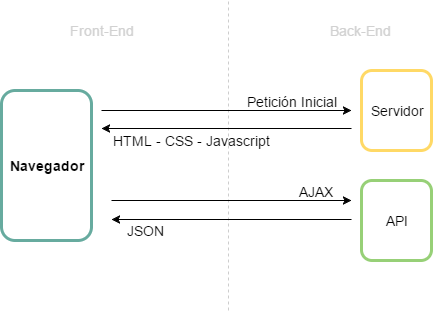
\includegraphics[scale=0.6]{spa_lifecycle.png}
\captionof{figure}{Ciclo de vida de una aplicación SPA}
\label{fig:spa_lifecycle}
\end{center}
\bigbreak
El ciclo de una aplicación SPA como se muestra en la \textbf{Figura \ref{fig:spa_lifecycle}} requiere por lo general una primera petición para cargar las vistas, funciones y diseño, el resto de las peticiones se dirigen al API a través de AJAX para pedir los datos a visualizar.

A continuación presentaremos dos (2) bibliotecas que nos permiten definir la aquitectura de la aplicación: Angular y jQuery.

\subsection{Angular}
Angular\footnote{Angular 2 \url{https://angular.io/}} es un framework muy popular creado por Google destinado a construir aplicaciones web, donde se maneja la lógica de la aplicación con JavaScript. Para la versión 2 de Angular, que es la que se contempla para este proyecto, se logra una estructura modular en la aplicación, donde cada elemento es considerado un componente que se construye de manera aislada, por lo tanto no se ve afectado por el resto de los mismos. Claramente, el enfoque de Angular sigue la arquitectura SPA, donde logra optimizar y resolver posibles problemas con los estados de transiciones, carga inicial, caching y mejor manejo de peticiones HTTP.

Es importante saber que Angular es una biblioteca con un catálogo inmenso de funcionalidades soportado por la mayoría de los navegadores, donde ofrece desde mecanismos de seguridad para evitar \textit{Cross-site scripting}\footnote{Cross-site scripting \url{https://es.wikipedia.org/wiki/Cross-site_scripting}} (XSS) hasta un paquete completo de animaciones.

A continuación, se muestra un ejemplo de código representando un componente en Angular:
\begin{lstlisting}
// app.component
import { Component } from '@angular/core';

@Component({
  selector: 'my-app',
  template: `<h1>Hola Mundo</h1>`
})
export class AppComponent { name = 'Angular'; }
\end{lstlisting}

Podemos observar que para declarar un componente es necesario importar primero el paquete de Angular y luego llamar al decorador \textbf{@Component({})}, en donde es pasado un objeto identificado por un \textbf{selector}, que corresponde a un alias del componente y el \textbf{template} que puede ser una ruta de un archivo HTML o este caso una pieza de código HTML.

\begin{lstlisting}
// app.module
import { NgModule }      from '@angular/core';
import { BrowserModule } from '@angular/platform-browser';
import { AppComponent }  from './app.component';

@NgModule({
  imports:      [ BrowserModule ],
  declarations: [ AppComponent ],
  bootstrap:    [ AppComponent ]
})
export class AppModule { }
\end{lstlisting}

Es indispensable al menos un módulo en Angular por lo tanto en el código anterior estamos definiendo un módulo con el decorador \textbf{@NgModule({})}, lo importante de aquí es que en dicho módulo declaramos el componente anteriormente creado.

Otras características que destacan a Angular son:

\begin{itemize}
\item\textbf{Directivas}

Es una manera de lograr que las vistas sean dinámicas, es decir, los componentes HTML pueden tener atributos especiales de Angular para poder modificar elementos del DOM.
\begin{lstlisting}
<li *ngFor="let item of arrayItem"></li>
<app-detail *ngIf="selectedItem"></app-detail>
\end{lstlisting}
La directiva \textbf{*ngFor} nos permite iterar en un ciclo, originando un <li> por cada elemento de arrayItem y \textbf{*ngIf} nos permite mostrar o no elementos mediante una condición.

\item\textbf{Servicios}

Pueden representar cualquier función, valor o características que la aplicación necesite. Mayormente los componentes son consumidores de estos servicios, por ejemplo: una configuración de la aplicación, un servicio que hace peticiones HTTP a un API, un servicio encargado de actualizar una barra de navegación, un servicio para mostrar mensajes estilo Logs, etc.
\begin{lstlisting}
// logger.service.ts
export class Logger {
  log(msg: any)   { console.log(msg); }
  error(msg: any) { console.error(msg); }
  warn(msg: any)  { console.warn(msg); }
}
\end{lstlisting}
El código de arriba representa un ejemplo de un servicio de Logs, en donde nos ofrece una clase con tres (3) variedades de avisos a consola.
\end{itemize}

\subsection{jQuery}
jQuery\footnote{jQuery \url{https://jquery.com/}} es una biblioteca ligera y sencilla, que lleva bastante tiempo siendo usada. Su finalidad es ofrecer soluciones a funciones complejas de manera sencilla principalmente para la manipulación de elementos HTML y eventos, animaciones y AJAX. Considero jQuery como una opción manual al construir una aplicación SPA, ya que directamente no ofrece una solución completa, pero existen plugins y/o guías para lograr dicha arquitectura.

\begin{itemize}

\item\textbf{Manipulación de elementos}
\begin{lstlisting}
$( "button.green" ).html( "Next" );
\end{lstlisting}

\item\textbf{Manejo de Eventos}
\begin{lstlisting}
var hiddenBox = $( "#banner-message" );
$( "#button-container button" ).on( "click", function( event ) {
  hiddenBox.show();
});
\end{lstlisting}

\item\textbf{Petición HTTP Asíncrona con AJAX}
\begin{lstlisting}
$.ajax({
  url: "/api/getWeather",
  data: {
    zipcode: 97201
  },
  success: function( result ) {
    $( "#weather-temp" ).html( "<strong>" + result + "</strong> degrees" );
  }
});
\end{lstlisting}
\end{itemize}

\section{Diseño}

Es importante que nuestra aplicación presente un buen diseño, donde se simplifique la finalidad de la aplicación, además de ser capaz a adaptarse a distintos tamaños de pantallas. No hay un guion o estilo definido para el diseño, la idea es aplicar colores que combinen, componentes sencillos como: botones, selectores, barra de menú, diálogos, iconos, \textit{inputs} (entradas de información), texto y componentes no tan sencillos como las gráficas para visualizar los datos. Todos estos componentes harán posible una interfaz que sea capaz de representar un editor de visualizaciones, en donde recibiremos apoyo de bibliotecas que nos ofrecen estos componentes bien formados y listos para usar.

\subsection{Angular Material}

Angular Material\footnote{Angular Material \url{https://material.angular.io/}} es una biblioteca que ofrece componentes siguiendo un diseño llamado Material (Material Design)\footnote{Material Design \url{https://material.io/}} creado por Google. Para poder integrar esta biblioteca es requerido Angular 2, por lo tanto, esta opción se ve atada a usar dicho framework. Lo que destaca de Angular Material es la variedad de componentes, que además son totalmente adaptativos gracias a una biblioteca incluida llamada \textit{Flex Layout}\footnote{Flex Layout \url{https://github.com/angular/flex-layout}} que nos ofrece propiedades sencillas de usar para corresponder el tamaño de los componentes en distintos escenarios. Adicionalmente, es soportado por la mayoría de los navegadores modernos.

Angular Material al estar atado al framework nos da la posibilidad de exportar sólo los componentes que necesitemos y no todos los de la biblioteca, además nos permite añadir soporte de gestos a los componentes como \textit{toggle} o \textit{slider}.

Entre tantos componentes, se mostrará ejemplos de algunos a continuación:

\begin{itemize}
\item\textbf{Botones}
\begin{lstlisting}
<button md-raised-button>Raised button</button>
<button md-fab><md-icon>check</md-icon></button>
\end{lstlisting}
En donde el atributo \textbf{md-raised-button} representa un botón con elevación, \textbf{md-fab} es un botón mayormente flotante con forma circular. Podemos observar que existe otro elemento \textbf{md-icon} que nos permite colocar un ícono a través de una fuente especial llamada \textit{Material Design Icons}\footnote{Material Design Icons \url{https://material.io/icons/}}, obteniéndola con el siguiente código desde nuestro archivo HTML.
\begin{lstlisting}
<link href="https://fonts.googleapis.com/icon?family=Material+Icons" rel="stylesheet">
\end{lstlisting}

\item\textbf{Spinner de Progreso}
\begin{lstlisting}
<md-progress-spinner
    class="example-margin"
    [attr.color]="color"
    [mode]="mode"
    [value]="value">
</md-progress-spinner>
\end{lstlisting}
El \textit{spinner}, que hace referencia a un elemento circular con acción de progreso, se puede lograr usando \textbf{md-progress-spinner} en donde puede tener como atributo un color, un modo para representar si girará finitamente o infinitamente y un valor que representa el porcentaje de progreso actual.

\item\textbf{Barra de Herramientas}
\begin{lstlisting}
<md-toolbar>My App</md-toolbar>
\end{lstlisting}
Con \textbf{md-toolbar} logramos crear una barra en donde podremos colocar texto e iconos con acciones, por ejemplo, la barra principal superior de la aplicación.
\end{itemize}


\subsection{Bootstrap}

Bootstrap\footnote{Bootstrap \url{http://getbootstrap.com/}} ofrece un gran catálogo de componentes, desde distintos tipos de botones, formularios, barras de menú, hasta diálogos. Recientemente lanzaron la versión 4, en donde se reescribió la mayoría del proyecto corrigiendo bastantes errores, sin embargo esta versión se encuentra en fase alfa, esto quiere decir que no es estable. Bootstrap es una biblioteca elaborada por Twitter, donde es posible la construcción rápida de una interfaz tanto para escritorio como para móvil, ofreciendo gran soporte para la mayoría de los navegadores y también posibilidad de adaptarse a distintas dimensiones de pantallas. Para que Bootstrap funcione es necesario la biblioteca jQuery que anteriormente mencionamos.

Bootstrap tienen su propio sistema \textit{grid} para escalar los componentes según cambie el tamaño de la pantalla, en donde se distinguen tres medidas: \textbf{lg} (largo), \textbf{md} (mediano), \textbf{sm} (pequeño) y \textbf{xs} (extra pequeño). Estas medidas pueden aplicarse a columnas o filas, representadas como \textbf{col} y \textbf{row}. Por cada fila puede haber doce (12) columnas, si este es superado el elemento faltante irá posicionado abajo.
\begin{lstlisting}
<div class="row">
  <div class="col-md-4">.col-md-4</div>
  <div class="col-md-4">.col-md-4</div>
  <div class="col-md-4">.col-md-4</div>
</div>
<div class="row">
  <div class="col-xs-12 col-md-8">.col-xs-12 .col-md-8</div>
  <div class="col-xs-6 col-md-4">.col-xs-6 .col-md-4</div>
</div>
\end{lstlisting}

Entre los componentes considerados a usar:
\begin{itemize}
\item\textbf{Botones}
\begin{lstlisting}
<button type="button" class="btn btn-default">Default</button>
<button type="button" class="btn btn-primary">Primary</button>
<button type="button" class="btn btn-success">Success</button>
<button type="button" class="btn btn-info">Info</button>
<button type="button" class="btn btn-warning">Warning</button>
<button type="button" class="btn btn-danger">Danger</button>
\end{lstlisting}
Bootstrap nos proporciona un abanico de botones con estilos definidos, en donde cada uno juega un color de fondo distinto.

\item\textbf{Tipografía}
\begin{lstlisting}
<span class="glyphicon glyphicon-star" aria-hidden="true"></span> Star
\end{lstlisting}
Es posible incluir íconos gracias a que Bootstrap trae su propia tipografía.

\item\textbf{Barra de Progreso}
\begin{lstlisting}
<div class="progress">
  <div class="progress-bar" role="progressbar" aria-valuenow="60" aria-valuemin="0" aria-valuemax="100" style="width: 60%;">
    <span class="sr-only">60% Complete</span>
  </div>
</div>
\end{lstlisting}

\item\textbf{Barra de Herramientas}
\begin{lstlisting}
<nav class="navbar navbar-default">
  <div class="container-fluid">
    <div class="navbar-header">
      <a class="navbar-brand" href="#">
        <img alt="Brand" src="...">
        <h1>Title</h1>
      </a>
    </div>
  </div>
</nav>
\end{lstlisting}
Es posible posicionar una barra superior de manera fija, con cualquier elemento adentro de ella, pero para ellos debes cumplir con los 3 primeros elementos padres: el primer \textbf{nav} y los dos siguientes \textbf{div}.

\end{itemize}


\section{Utilidades}

Existen distintas bibliotecas de propósito más específico cuyo uso se ha vuelto cotidiano, donde pueden solucionar tareas complejas o engorrosas de implementar en JavaScript, específicamente para nuestro proyecto existe la necesidad de preparar ciertos conjuntos de datos complejos para poder construir una gráfica, al igual que manejar varios formatos de fechas.

\subsection[Lodash]{Lodash\footnote{Lodash \url{https://lodash.com/}}}

La manipulación de ciertos objetos, arreglos y strings complejos pueden contemplar soluciones un tanto ilegible, por lo tanto la biblioteca Lodash nos otorga utilidades que resuelven dichos problemas de una manera simple. Adicionalmente, cuenta con funciones matemáticas y soluciones para manejar valores null, NaN y undefined. Todas sus funcionalidades son soportadas por la mayoría de los exploradores.

A continuación, se mostrarán unos ejemplos de las ventajas que puede traer lodash a nivel de implementación:

\begin{itemize}
\item\textbf{Verificar variable (no sea null ni undefined)}
\begin{lstlisting}
// no-lodash
if(a != null && a != undefined) {...}

// lodash
if(!_.isNill(a)) {...}
\end{lstlisting}

\item\textbf{Ciclos}
\begin{lstlisting}
// no-lodash
for(var i = 0; i < 5; i++) {
  ...
}

// lodash
_.times(5, function(){
  ...
});
\end{lstlisting}

\item\textbf{Números aleatorios}
\begin{lstlisting}
// no-lodash
Math.floor(Math.random() * (max - min + 1)) + min;

// lodash
_.random(min, max);
});
\end{lstlisting}

\item\textbf{Seleccionar elementos de un arreglo}
\begin{lstlisting}
// no-lodash
function pick(arr) {
    var _this = this;
    var obj = {};
    arr.forEach(function(key){
        obj[key] = _this[key];
    });

    return obj;
};
objA.pick(['x', 'y'])

// lodash
_.pick(objA, ['x', 'y']);
});
\end{lstlisting}
\end{itemize}

\subsection[Moment]{Moment\footnote{Momentjs \url{https://momentjs.com/}}}

La manipulación de fecha y tiempo en JavaScript suele ser confusa y consume muchas líneas de código, es probable que en nuestra aplicación tengamos que recibir fechas con un formato específico y de la misma forma representar este visualmente de otra. Moment es una biblioteca que tiene como finalidad analizar sintácticamente, validar, manipular y mostrar fechas/horas (tiempo) de la forma más simple posible. Adicionalmente, esta biblioteca ofrece extensiones para poder realizar ciertas funcionalidades más específicas.

A continuación mostraremos ejemplos de cosas interesantes que podemos lograr con dicha biblioteca:

\begin{itemize}
\item\textbf{Obtener la fecha/hora de hoy con formato}
\begin{lstlisting}
// date
moment().format("DD/MM/YYYY");
// time
moment().format("HH:mm:ss");
\end{lstlisting}

\item\textbf{Agregar/Quitar tiempo}
\begin{lstlisting}
// add
moment().add(7, 'days');
moment().add(1, 'week')
// subtract
moment().subtract(7, 'days');
moment().subtract(1, 'week')
\end{lstlisting}

\item\textbf{Obtener unidad de tiempo específica}
\begin{lstlisting}
// hours
moment().hours();
// month
moment().month();
\end{lstlisting}
\end{itemize}